\section{Multi-player flowchart and explanation~\ref{fig:multiplayer}}

\begin{figure}
    \centering 
    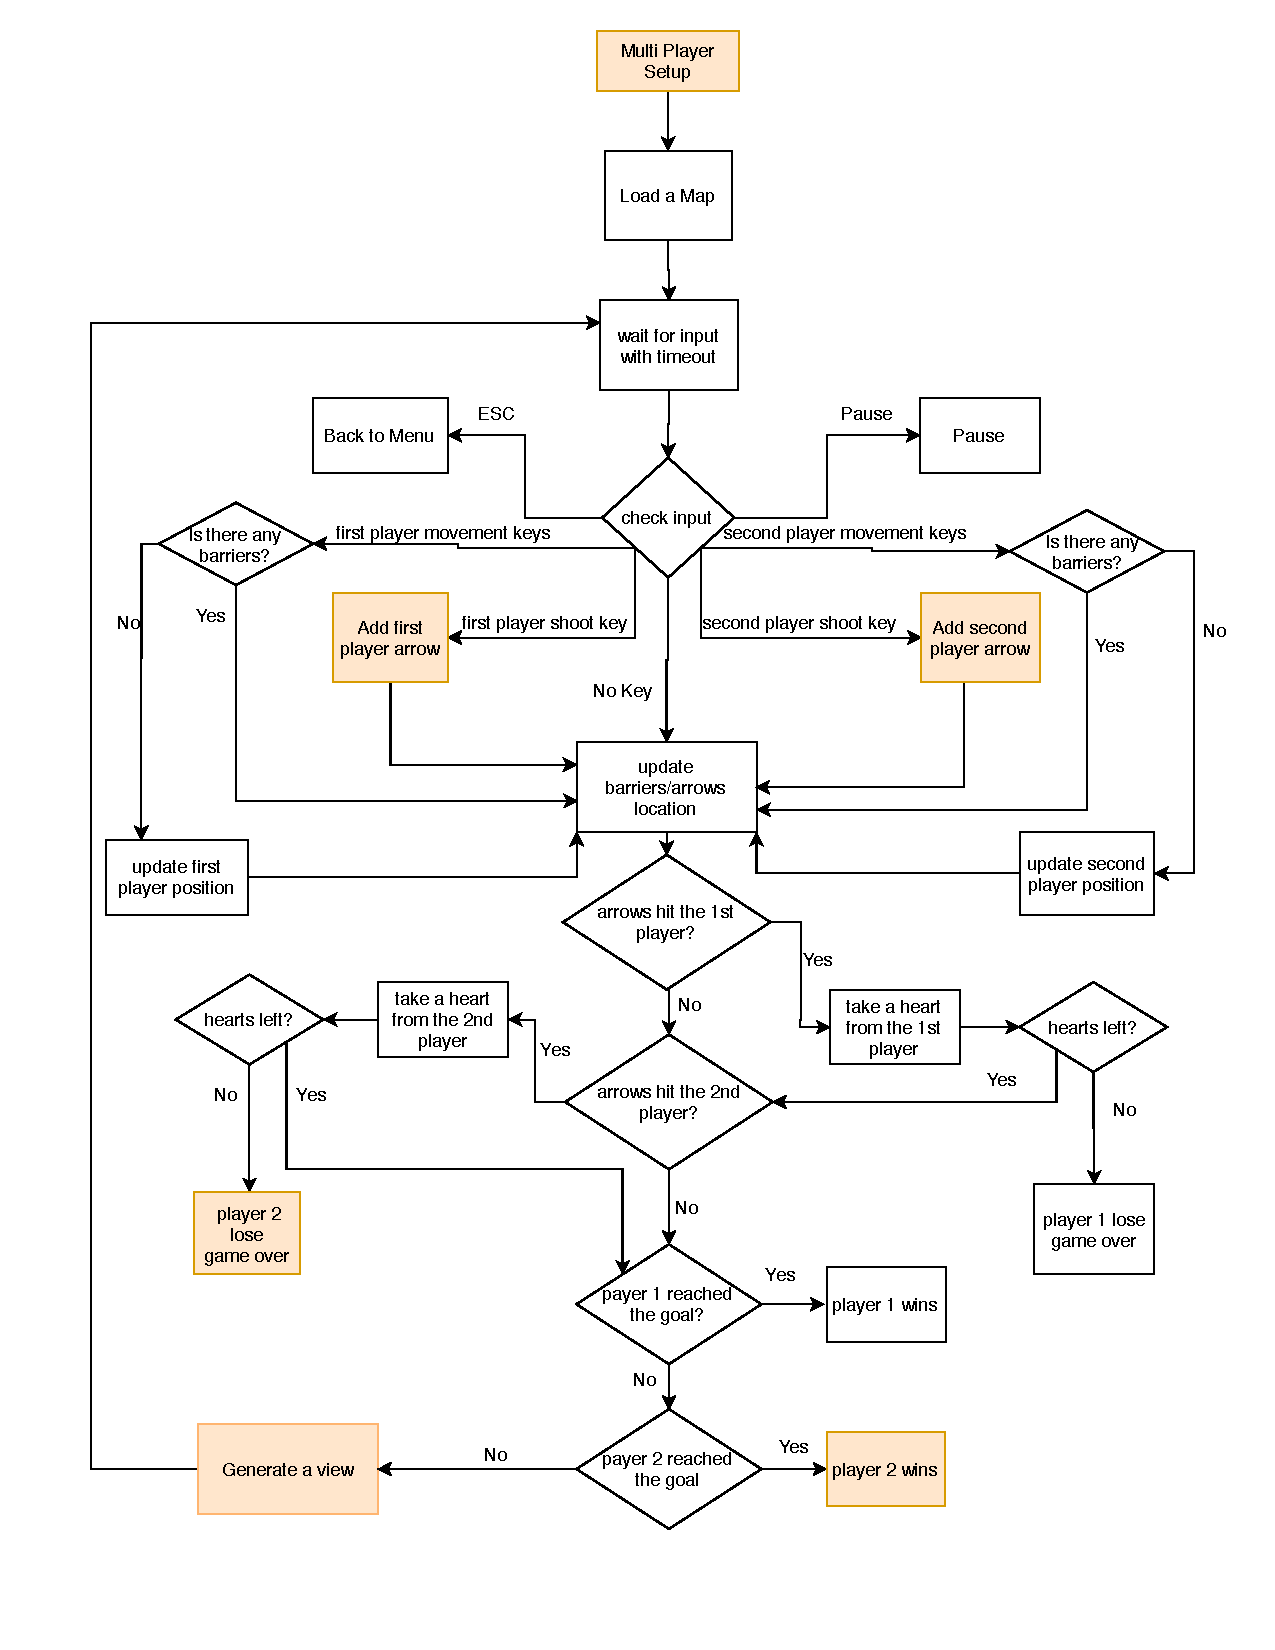
\includegraphics[width=0.9\columnwidth]{multiplayer.pdf}
    \caption{Multi-player block flowchart. Blocks which are in \textcolor{orange}{orange} will be implemented for the second release. Some functions and blocks are used in both single player and multi-player mode which are in white color.}
    \label{fig:multiplayer}
\end{figure}

This Flow chart explains all the steps happening on s multi-player mode. 
As it is shown in Figure~\ref{fig:multiplayer}, after we select the multi-player option in Menu function, we begin from the load Map step, where we should read the map from a text file. 
Next, we do some setups for multi-player game based on the map. 
In these setups, we define a map with positions of two players, the goal, the barriers and the arrows. 
We should then get input from keyboard. 
We should check if there was any input given for either player. 
If not, we should update the position of barriers/arrows as they are moving objects. 
If either player hits escape button, we go back to menu. 
If hits pause button, we go to the state of pause game. 
If hits continue, we should continue the game. 
In both continue and pause state, we go back to get input from keyboard and wait for either player to enter another key. 
Given the movement keys, we update the position of first/second player accordingly. 
Also, by giving the specific shoot keys, we then generate arrows from the position of the shooting player. 
Both players need to run in different directions controlled by movement keys to avoid being shot by moving arrows. 
The process of dealing with barriers, losing hearts and reaching the goal for each player is the same as single player mode. 
By continuing to check the remaining hearts of them during the whole movement, we can know which player loses the game earlier than the other, which is the same way as judging whether the game is over for single player mode. 
As for the win scenario, only if the play alive reaches the final goal. 
If not reaching the win state ever, the program will generate a view afterwards and continue the problem waiting for another key input.

\subsection{Multi-player functions prototypes}

In this section we define the required functions prototypes and its relation to flow chart~\ref{fig:singleplayer}. We define some functions and the rest of the code will be in a main function. Comments above each function mention the associated block, the release, and assignee. Some functions are in common for both single player and multi-player mode.We just mention these functions as they already described and assigned and introduced new functions for the rest of this part.

\begin{minted}{c}
/* Functions created in first release and will be used in the second release */
Map loadMap(FILE* file_p);
void backToMenu(void);
void pauseGame(void);
int isBarrier(Player player,MapBarrier* barrier);
void updateArrow(MapArrow* arrow, MapSpace space);
void updateBarrier(MapBarrier* barrier, MapSpace space);
void updatePlayerPos(Player *player, int arrowKey);
int isPlayerHit(Player player, MapArrow* arrow );
void lostHeart(Player player);
int reachGoal(Player player, Goal goal);
int isGameOver(Player player);
void gameOver(Player player);
void winGame(Player player);

/* Created in the first release and updated in the second release*/
void updateView(Map map);

/* New functions*/
/* Block: Add first player arrow, Add second player arrow - second release
 * Assigned to: Mahsa
 * Generates an arrow and add it to the list of the arrows in the map
 * Input: player, map_p
 * Output: updated map_p
 * Return: void */
void shoot(Player player, Map* map_p);
\end{minted}